\documentclass{beamer}
\usepackage{ArmenianSlides}

\begin{document}

\title[Command]{Նախագծման Ձևանմուշներ։ Command}
\author[Հրաչյա Թանդիլյան\copyright]{Հրաչյա Թանդիլյան}
\date{2020}

%-------------------------------------------------------------------------------------------------
\begin{frame}
\titlepage
\end{frame}
%-------------------------------------------------------------------------------------------------

\section{Նպատակը}
%-------------------------------------------------------------------------------------------------
\begin{frame}\frametitle{Command}
\begin{block}{Նպատակը}
    Հարցումը ինկապսուլացնել օբյեկտի մեջ, դրանով իսկ թույլ տալ օբյեկտները տարբեր
    հարցումներով պարամետրիզացնել, կազմել հարցումերի հերթեր, գրանցել հարցումները (log),
    իրականացնել վերականգնելի (undoable) գործողություններ:
\end{block}
\vfill
Նաև հայտնի է որպես
\begin{itemize}
    \item Action
    \item Transaction
\end{itemize}
\end{frame}
%-------------------------------------------------------------------------------------------------

\subsection{Մոտիվացիան}
%-------------------------------------------------------------------------------------------------
\begin{frame}\frametitle{Մոտիվացիան}
\begin{center}
    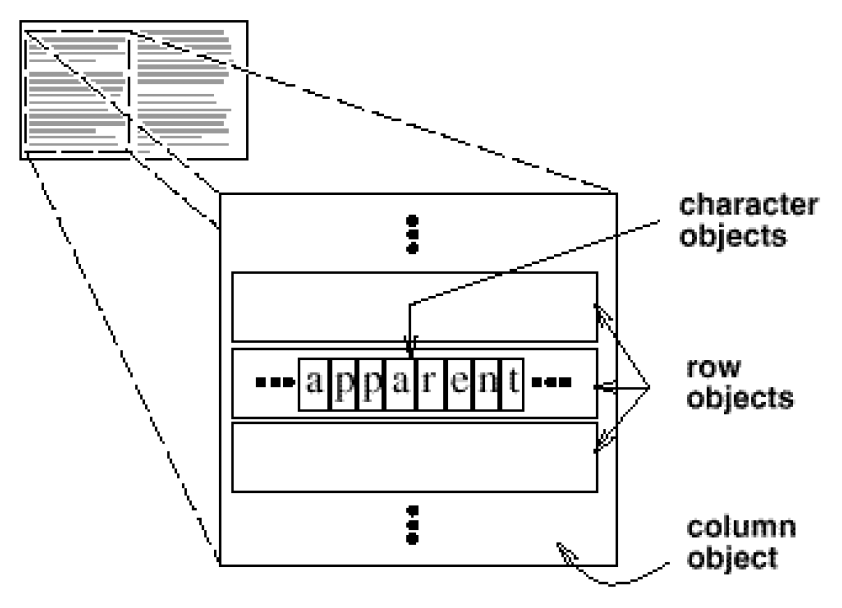
\includegraphics[scale=0.4]{motivation1.png}
\end{center}
\end{frame}
%-------------------------------------------------------------------------------------------------

%-------------------------------------------------------------------------------------------------
\begin{frame}\frametitle{Մոտիվացիան}
\begin{center}
    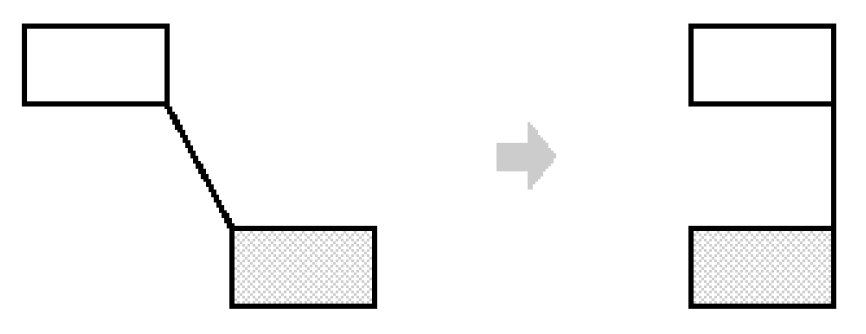
\includegraphics[scale=0.4]{motivation2.png}
\end{center}
\end{frame}
%-------------------------------------------------------------------------------------------------

%-------------------------------------------------------------------------------------------------
\begin{frame}\frametitle{Մոտիվացիան}
\begin{center}
    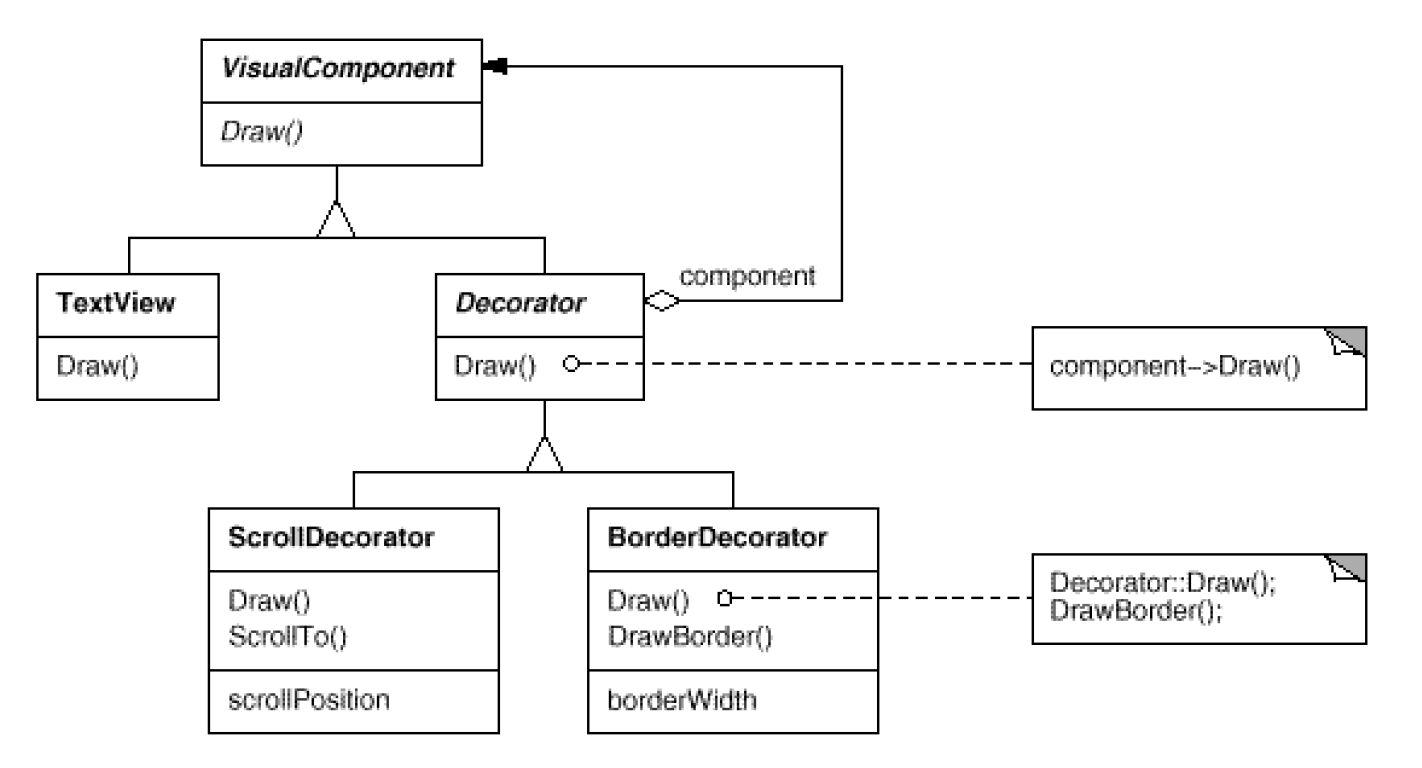
\includegraphics[scale=0.4]{motivation3.png}
\end{center}
\end{frame}
%-------------------------------------------------------------------------------------------------

%-------------------------------------------------------------------------------------------------
\begin{frame}\frametitle{Մոտիվացիան}
\begin{center}
    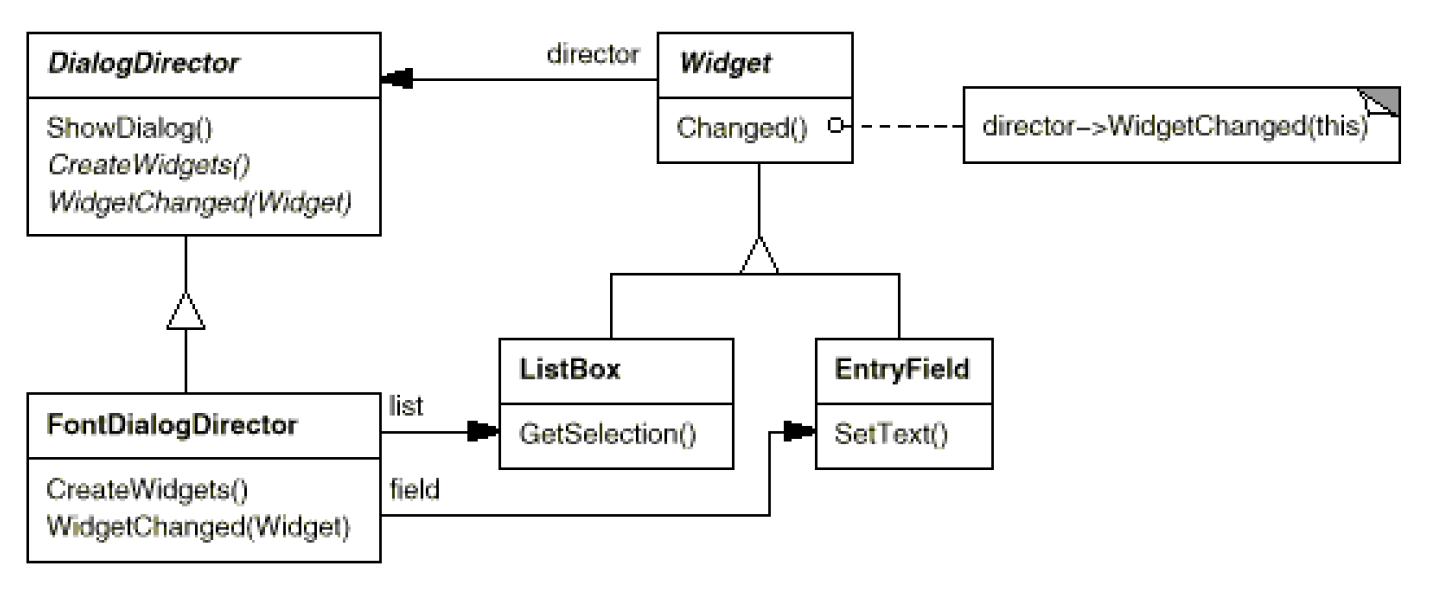
\includegraphics[scale=0.4]{motivation4.png}
\end{center}
\end{frame}
%-------------------------------------------------------------------------------------------------

\subsection{Կիրառելիությունը}
%-------------------------------------------------------------------------------------------------
\begin{frame}\frametitle{Կիրառելիությունը}
Այս Ն.Ձ. պետք է օգտագործել երբ.
\vfill
\begin{enumerate}
    \scriptsize
    \item Անհրաժեշտ է օբյեկտները պարամետրիզացնել կատարվելիք գործողությունով:
    Հանդիսանում է պրոցեդուրալ լեզուներում կիրառվող callback ֆունկցիաի օբյեկտային
    համարժեքը: \pause \vfill
    \item Անհրաժեշտ է հարցումները տալ, հավաքել և կատարել ժամանակի տարբեր
    պահերի: \pause \vfill
    \item Անհրաժեշտ է տրամադրել undo գործողություն: \pause \vfill
    \item Անհրաժեշտ է գրանցել փոփոխությունները այնպես, որ դրանք հնարավոր լինի
    կրկնել համակարգի աշխատանքի խափանման պարագայում:
\end{enumerate}
\end{frame}
%-------------------------------------------------------------------------------------------------

\section{Կառուցվածքը}
%-------------------------------------------------------------------------------------------------
\begin{frame}\frametitle{Կառուցվածքը}
\begin{center}
    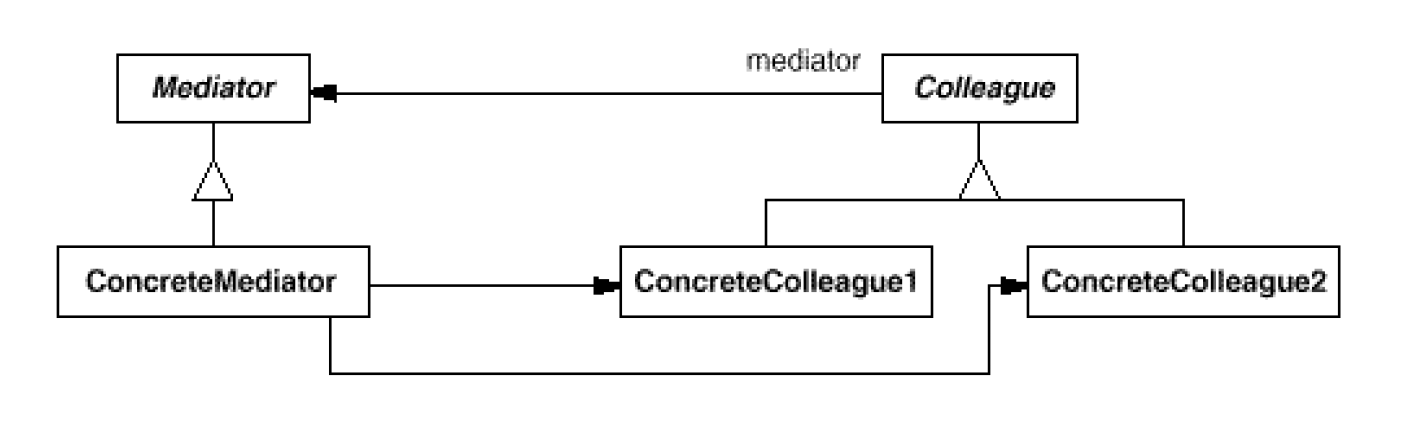
\includegraphics[scale=0.4]{structure1.png}
\end{center}
\end{frame}
%-------------------------------------------------------------------------------------------------

%-------------------------------------------------------------------------------------------------
\begin{frame}\frametitle{Կառուցվածքը}
\begin{center}
    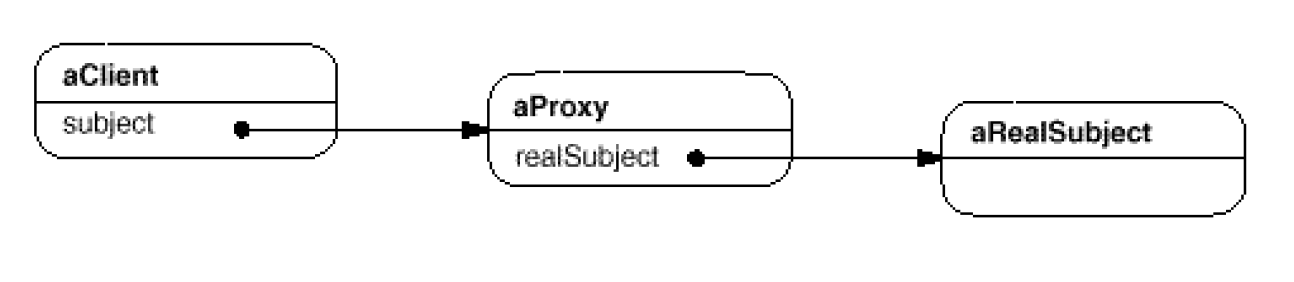
\includegraphics[scale=0.4]{structure2.png}
\end{center}
\end{frame}
%-------------------------------------------------------------------------------------------------

\subsection{Հետևանքները}
%-------------------------------------------------------------------------------------------------
\begin{frame}\frametitle{Հետևանքները}
Այս Ն.Ձ. ունի հետևյալ առավելություններն ու թերությունները.
\vfill
\begin{enumerate}
    \scriptsize
    \item Առանձնացնում է գործողության կանչն իրականացնող օբյեկտին այն օբյեկտից,
    որը գիտի թե ինչպես գործողությունը կատարել: \pause \vfill
    \item Քանի որ գործողությունը մոդելավորվում է սովորական օբյեկտի միջոցով,
    այն կարելի է ղեկավարել և ընդլայնել այլ օբյեկտների նման: \pause \vfill
    \item Հրամաններ կարելի է հավաքել կոմպոզիտ հրամանների մեջ: \pause \vfill
    \item Նոր տիպի գործողությունների ավելացումը հեշտ է, քանի որ գոյություն ունեցող
    գործողությունները փոփոխելու անհրաժեշտություն չկա:
\end{enumerate}
\end{frame}
%-------------------------------------------------------------------------------------------------

\section{Իրականացումը}
%-------------------------------------------------------------------------------------------------
\begin{frame}\frametitle{Իրականացումը}
\begin{enumerate}
    \item Որքան խելացի պետք է լինի Command-ը: \vfill
    \item Undo / Redo գործողությունների իրականացում: \vfill
    \item Undo / Redo գործողությունների կատարման ժամանակ սխալի կուտակում: \vfill
    \item C++-ի template-ների կիրառում:
\end{enumerate}
\end{frame}
%-------------------------------------------------------------------------------------------------

\subsection{Օրինակ}
%-------------------------------------------------------------------------------------------------
\begin{frame}[fragile]\frametitle{Օրինակ}
\begin{english}
\begin{minted}{cpp}
class Command {

public:
    virtual ~Command();
    virtual void Execute() = 0;

protected:
    Command();
};
\end{minted}
\end{english}
\end{frame}
%-------------------------------------------------------------------------------------------------

%-------------------------------------------------------------------------------------------------
\begin{frame}[fragile]\frametitle{Օրինակ}
\begin{english}
\begin{minted}[fontsize=\scriptsize]{cpp}
class OpenCommand : public Command {

public:
    OpenCommand(Application* a) : application(a) {}
    virtual void Execute() {
        const char* name = AskUser();
        if (name != 0) return;

        Document* document = new Document(name);
        application->Add(document);
        document->Open();
    }

protected:
    virtual const char* AskUser();

private:
    Application* application;
    char* response;
};
\end{minted}
\end{english}
\end{frame}
%-------------------------------------------------------------------------------------------------

%-------------------------------------------------------------------------------------------------
\begin{frame}[fragile]\frametitle{Օրինակ}
\begin{english}
\begin{minted}{cpp}
class PasteCommand : public Command {

public:
    PasteCommand(Document*) document(doc) {}

    void PasteCommand::Execute () {
        document->Paste();
    }

private:
    Document* document;
};
\end{minted}
\end{english}
\end{frame}
%-------------------------------------------------------------------------------------------------

%-------------------------------------------------------------------------------------------------
\begin{frame}[fragile]\frametitle{Օրինակ}
\begin{english}
\begin{minted}{cpp}
template <class Receiver>
class SimpleCommand : public Command {

public:
    typedef void (Receiver::* Action) ();

    SimpleCommand(Receiver* r, Action a)
        : receiver(r), action(a) {}

    virtual void Execute() {
        (receiver->*action)();
    }

private:
    Action action;
    Receiver* receiver;
};
\end{minted}
\end{english}
\end{frame}
%-------------------------------------------------------------------------------------------------

%-------------------------------------------------------------------------------------------------
\begin{frame}[fragile]\frametitle{Օրինակ}
\begin{english}
\begin{minted}{cpp}
MyClass* receiver = new MyClass;

Command* aCommand = new SimpleCommand<MyClass>(receiver,
                                               &MyClass::Action);
aCommand->Execute();
\end{minted}
\end{english}
\end{frame}
%-------------------------------------------------------------------------------------------------

%-------------------------------------------------------------------------------------------------
\begin{frame}[fragile]\frametitle{Օրինակ}
\begin{english}
\begin{minted}[fontsize=\scriptsize]{cpp}
class MacroCommand : public Command {

public:
    MacroCommand();
    virtual ~MacroCommand();

    virtual void Add(Command*) { cmds->Append(c); }
    virtual void Remove(Command*) { cmds->Remove(c); }

    virtual void Execute() {
        ListIterator<Command*> i(cmds);
        for (i.First(); !i.IsDone(); i.Next()) {
            Command* c = i.CurrentItem();
            c->Execute();
        }
    }

private:
    List<Command*>* cmds;
};
\end{minted}
\end{english}
\end{frame}
%-------------------------------------------------------------------------------------------------

\section{Առնչվող Ձևանմուշները}
%-------------------------------------------------------------------------------------------------
\begin{frame}\frametitle{Առնչվող Նախագծման Ձևանմուշները}
\begin{itemize}
    \item Composite \vfill
    \item Memento \vfill
    \item Prototype
\end{itemize}
\end{frame}
%-------------------------------------------------------------------------------------------------

\end{document}
